\chapter{Evolutionary Algorithms}\label{chapter_ea}\index{Evolutionary Algorithms}

\noindent This chapter provides the reader with a comprehensive overview of what evolutionary algorithms entail along with a representative selection of existing work. An introduction to evolutionary algorithms is first given in Section \ref{ea_introduction}. Section \ref{historical_background} paints a picture of the historical background of evolutionary algorithms. The reader is then provided with fundamentals behind evolutionary algorithms in Section \ref{sec:ea_core_concepts}. Section \ref{sec:ea_types_of_ea} reviews the different evolutionary algorithms that exist and their differences, and finally Section \ref{sec:ea_current_research} provides an overview of current advancements in the field of evolutionary computation.

\section{Introduction}\label{ea_introduction}
Evolutionary Algorithms (EAs) belong to a large group of optimisation methods that take inspiration from Darwinian biological evolution (\cite{book_introduction_to_evolutionary_computing}). These methods replicate processes like natural selection, mutation, and reproduction. They simulate the adaptive and competitive dynamics observed in nature, where a set of candidate solutions, called the population, is iteratively refined over multiple generations (\cite{basicsOfEvolutionaryComputing}). 

\parbreak\noindent In order to mimic the lifecycle of organisms, selecting a representation of a candidate solution that is amenable to algorithmic manipulation is a prerequisite. With the proper representation of a candidate solution in place, EAs follow the general framework of mimicking the lifecycle of organisms. To explain simply, this framework works firstly by generating an arbitrary number of handful candidate solutions that make up the initial population. Each candidate solution will have an attempt at solving the problem at hand after which this attempt will be scored and recorded relative to a particular fitness. This scoring scheme is achieved by a \textit{fitness function} and generally has the primary role of determining how strong an individual is at solving the problem at hand. Each candidate solution will then go through a selection process whereby the best solution will be chosen, and the others disregarded, ensuring that only the best-performing candidates pass their desirable traits onto offspring and consequently forthcoming generations. Additionally, a mechanism is established to combine candidate solutions, facilitating the exchange of traits to enhance the diversity and quality of the population over successive iterations. Surviving candidates will produce offspring by applying genetic operators such as mutation (which introduces variability by altering the gene of offspring) and crossover (which combines the traits from two or more parents). After population initialization, this repetitive process of selection, mutation, and reproduction enhances the likelihood that the successive generations migrate towards a global optima while mitigating the chances of falling into a local optima (\cite{evolutionaryComputingAndNeuralNetworks}). 

\parbreak\noindent EAs have been applied to a wide range of different fields ranging from engineering, to artificial intelligence. EAs are typically used in optimisation problems where there is a single or multiple objectives due to their ability to explore the solution space in a flexible manner. EAs have application in a vast number of fields where for example EA algorithms were used to optimise solar panel layouts in real-time by aircrafts in the engineering realm. Another example was EAs involvement to predict flood routing in natural channels using gene expression programming (GEP) in the environmental field (\cite{slowik2020evolutionary}).

\section{Historical Background}\label{historical_background}
EAs go back to the early computational era of the 1950s and 60s where researchers began to draw inspiration from Darwinian principles of natural selection (\cite{alainsanaEvolutionaryAlgorithms}). These researchers managed to mathematically model the competitive and adaptive processes found in nature in order to solve and optimise complex and multi-dimensional problems. The idea was simple - just as organisms in nature evolve to adapt according their environment, organisms in the mathematical realm (candidate solutions) can \textit{"evolve"} by competing and improving over time, akin to  natural generations. This approach in solving optimisation problems became compelling to be used in problems that were ill-defined or had far too many variables that lead to exhaustive searching and suboptimal solutions. 

\parbreak\noindent EAs began with contributions from many important people. British mathematical and geneticist Alex Fraser took early steps to model genetic ideas using computers in the 1950s (\cite{links2002alex}). Hans-Paul Schwefel and Ingo Rechcenberg were inspired by his work and soon developed evolution strategies in Germany during the 1960s primarily for application in engineering (\cite{alainsanaEvolutionaryAlgorithms}). Around that time, an American Scientist, John Holland, formulated the concept of genetic algorithms (GAs) which established a formal framework to simulate biological evolution in a mathematical sense. Holland's work in the 1970s revolutionized EAs extending their application in many areas (\cite{alainsanaEvolutionaryAlgorithms}). After the publication of the book, \textit{Genetic Algorithms in Search, Optimisation and Machine Learning} by E. Goldberg in 1989, interest in the field became much more widespread (\cite{alainsanaEvolutionaryAlgorithms}).

\parbreak\noindent As the field of computers evolved in terms of technological sophistication and breadth of application, so did the capabilities and appeal of evolutionary algorithms. Due to advancements in computer science in the late 20th century, researchers began to explore more complex and sophisticated EA models. Also PhD student of John Holland, John Koza, a computer science researcher, formulated genetic programming which opened new avenues for using evolution to optimise non\-linear structures such as symbolic regression functions and tree\-like structures (\cite{koza1994genetic}). Differential Evolution (DE) was introduced in the 1990s which provided a mechanism in solving problems suited for continuous parameter optimisation (\cite{das2010differential}).

\section{Core Concepts in Evolutionary Algorithms}\label{sec:ea_core_concepts}
EAs are built from several core concepts that mimic Darwinian principles, that is, the process of selection, variation, and inheritance. These core elements form the backbone of the way in which EAs operate, creating a system whereby candidate solutions are evolved over iterative generations to meet or exceed a given objective. Understanding these core concepts are crucial in understanding the mechanics and flexibility of EAs, as each component dictates how the algorithm explores and optimises the search space.

\parbreak
\begin{figure}[H] % Use [H] to suppress floating and place the figure/table exactly where it is specified in the text
	\centering % Horizontally center the figure on the page
	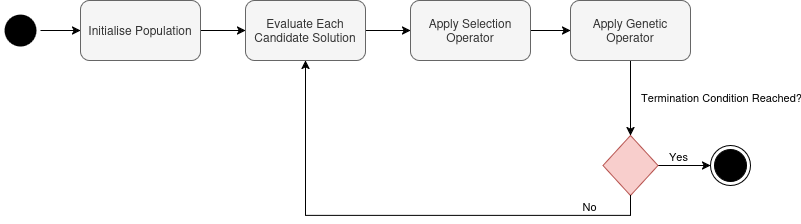
\includegraphics[width=\textwidth]{Figures/chapter_ea/chapter_ea_ea_framework.png} % Include the figure image
	\caption{Evolutionary Algorithm Framework (adapted from \cite{handsOnGeneticAlgorithms})}
	\label{fig:ea_framework} % Unique label used for referencing the figure in-text
\end{figure}

\subsection{Representation}
The term chromosome is often used to refer to representations of candidate solutions within the population which are a critical aspect of the evolutionary algorithms, an attempt to model genes and chromosomes seen in nature. The representation dictates how individuals are encoded, manipulated, and evaluated within the evolutionary process. A representation that is well-defined within the context of the optimisation problem enhances the algorithm's ability to explore the search space efficiently while maintaining diversity and feasibility among solutions.

\parbreak\noindent The genotype-phenotype mapping translates encoded information into a meaningful solution. There are two forms in an evolutionary algorithm, namely, the \textbf{genotype} which is the encoded representation of a solution and is typically manipulated directly by genetic operators such as crossover and mutation, and the \textbf{phenotype} which is the decoded, functional representation of the solution which is what gets evaluated against the fitness function or objective (\cite{okramergeneticalgorithms}). For example, consider an optimisation problem where a 4-bit binary number that decodes the highest integer value needs to be found. The genotype would be a chromosome representing a 4-bit string (e.g., $1010$). The phenotype would be the decoded integer value (e.g., $1010 \rightarrow 10$ in decimal). It is not necessarily for every optimisation problem to have an explicit genotype-phenotype mapping, in particular, when the genotype is the solution itself (\cite{okramergeneticalgorithms}).

\parbreak\noindent There are many ways in which chromosomes can be represented as solutions to the problem at hand. Representations are divided into two categories, namely, direct representations and indirect representations. Direct representations are those in which the genotype-phenotype mapping is one-to-one, allowing genetic operators to be applied directly without transformation. In contrast, indirect representations require an additional decoding step to map genotypes to phenotypes before genetic operators can be applied (\cite{rothlauf2009representations}). Genetic algorithms have originally been proposed to be binary coded to mimic the genetic material of natural organisms, however, different representations are used based contextually on the optimisation problem at hand (\cite{yu2010introduction}). Common representations include those seen in Figure \ref{fig:ea_representations}. Binary representations are commonly used for problems with discrete or combinatorial solutions, such as feature selection or Boolean optimisation, where each bit can encode the presence/absence of a feature or a binary decision. Integer or real-valued representations are suited for numerical optimisation tasks, such as parameter tuning in machine learning or engineering design, where variables require fine-grained precision. Tree-based representations model hierarchical structures, making them ideal for symbolic regression, program synthesis, or parsing tasks, where solutions naturally map to decision trees or recursive expressions.

\parbreak
\begin{figure}[h!] % Use [H] to suppress floating and place the figure/table exactly where it is specified in the text
	\centering % Horizontally center the figure on the page
	\includesvg[width=\textwidth]{Figures/chapter_ea/chapter_ea_representation.svg} % Include the figure image
	\caption{Common Gene Representation (adapted from \cite{intelligentOptimization})}
	\label{fig:ea_representations} % Unique label used for referencing the figure in-text
\end{figure}

\subsection{Population and Fitness}
The starting point in any evolutionary algorithm is the initialization of a population as shown in Figure \ref{fig:ea_framework} which represents a group of candidate solutions that could potentially solve the problem at hand. Unlike traditional optimisation techniques which mainly focus on a single-solution pathway, EAs work within the entire solution space by means of parallelism (\cite{okramergeneticalgorithms}). To put it simply, each generation evaluates candidate solutions as potential answers, with the algorithm progressively identifying better ones through selection and variation. This parallel search ensures that local optima are avoided, an issue which high-dimensional optimisation typically face. By ensuring that the initial population generated is diversified, there is an increased chance of finding a global or near global optimal solution. There are many methods for initializing a population, with randomized approaches being the most common, specifically those drawn from a uniform probability distribution, to ensure a broad coverage of the search space (\cite{initialPopulation}). Other mechanisms for initializing the population include heuristic and intelligent based approaches when existing solutions are known which could potentially ensure a better coverage spread of the search space (\cite{initialPopulation}). When taking advantage of using existing solutions to explore the search space, repetitive computations are mitigated yielding in an increased efficiency. Likewise, non-random initial populations can directly gear the algorithm to search a particular region of the solution space from the beginning which again, with the aid of known solutions, can allow the algorithm to converge quicker towards an optimal solution. Other mechanisms include deterministic based approaches in which candidate solutions are generated in a more controlled and evenly distributed manner leading to a better coverage of the solution space (\cite{THARWAT2021100952}).

\parbreak\noindent In genetic algorithms, diversity refers to the variety of genetic material (e.g., different solution features or values) within a population. The population's diversity closely relates to how well the candidate solutions explore the search space. If individuals are too similar, they lack diversity leading to premature convergence causing stagnation around a suboptimal solution. Conversely, if the individuals are too diverse from one another, convergence can be delayed meaning that more generations are needed in order to hone in on an optimal solution (\cite{okramergeneticalgorithms}). A fine balance is therefore needed between exploration and exploitation. A highly diverse initial population is crucial to ensure thorough exploration of the search space early in the optimisation process. As generations progress, the algorithm selectively converges toward higher-quality solutions, naturally reducing diversity while refining the best candidates. There are well studied mechanisms which can control this balance such as mutation rate adjustment, niche-reserving mechanisms, or even hybrid approaches. Using these mechanisms ensures that both diversity and convergence can be capitalized.

\parbreak\noindent With reference to Figure \ref{fig:ea_framework}, after the population is initialized, each candidate solution will be vetted by means of a fitness function which is a mathematical measure that scores how well the candidate solution meets the objective (\cite{okramergeneticalgorithms}). This score reflects the quality of the candidate solution in regard to the optimisation goal and is used to guide the selection process in subsequent generations. For example, given an optimisation problem such that $x$ is an integer to maximize the parabolic equation $f(x) = -x^2 + 25$, the fitness function would be taking a candidate solution, and feeding it as input into this equation. Evidently, the maximum fitness to this function would be $5$. Fitness functions are defined in different ways depending on the application at hand, for example, in engineering design problems, fitness may represent efficiency, structural stability, or cost-effectiveness, whereas in artificial intelligence, fitness could measure a predictive accuracy. The way in which a fitness function is defined shapes how effectively the EA converges towards an optimal solution, especially in multi-objective problems (MOPs) where the fitness needs to account for multiple goals (\cite{book_introduction_to_evolutionary_computing}).

\parbreak\noindent MOPs are mathematical problems that involve optimizing multiple conflicting objectives at the same time. The fitness function in this regard is defined by the algorithm's performance in relation to these conflicting objectives as opposed to one (\cite{okramergeneticalgorithms}). A common approach in formulating the fitness function is by aggregating all the objectives in a singular fashion by means of a weighted sum (\cite{okramergeneticalgorithms}). Another approach in defining the fitness function appropriately is by changing the structure of algorithm by means of co-evolution - instead of evolving a single population, the problem is broken down into smaller problems which in turn have their own population which is evolved (\cite{ZHOU201132}). In multi-objective optimisation problems which are common in economics and engineering, the fitness function may use methods like Pareto front optimisation which balances competing objectives without forcing single trade-off solutions. Pareto optimality describes a solution that cannot be improved in any objective without degrading another. In these kind of scenarios, EAs evolve a population of solutions that collectively represent a spectrum of optimal trade-offs, giving the decision-maker flexibility in choosing the most suitable solution based on contextual priorities (\cite{rachmawati2009multiobjective}). EAs are therefore robust and versatile in solving both single and multi-objective problems which can often be riddled with narrowly defined and complex optimisation challenges.

\subsection{Genetic Operators}\label{label:ea_genetic_operators}
In EAs, genetic operators - crossover and mutation - serves as crucial mechanisms by means of variation and adaption to guide the exploration of the solution space while refining existing solutions. Variation in evolution can be divided into two types based on their arity, namely, unary (mutation) and n-ary (recombination) both of which produce offspring (\cite{book_introduction_to_evolutionary_computing}). These operators mimic the evolutionary processes seen in nature among organisms, where gene recombination and mutation introduce new traits that contribute to a population's overall fitness and adaptability (\cite{handsOnGeneticAlgorithms}).

\subsubsection{Crossover}
Crossover is an evolutionary process based on sexual reproduction whereby genetic material from two parents are combined to produce offspring that inherit characteristics from both (\cite{okramergeneticalgorithms}). Crossover plays a crucial part in diversifying the algorithm's search path by combining beneficial traits and thereby ideally producing offspring with improved fitness. There are different ways in which crossover can occur which provide varying levels of control over the inheritance process. For simplicity, consider linear gene representations for the following crossover mechanisms.

\parbreak\noindent \paragraph{Single-point Crossover} selects a single point along the chromosome and exchanges genetic material on either side as shown in Figure \ref{fig:singlepoint}. This simple approach works well when minor structural adjustments results in significant improvement (\cite{intelligentOptimization}).

\parbreak\noindent \paragraph{Multi-point crossover} introduces more than one cutoff point, allowing for more complex combinations of genetic material from each parent thereby creating a more diverse offspring as shown in Figure \ref{fig:multipoint} (\cite{crossoverMethods}). Multi-point crossover is typically used in scenarios that are non-linear. 

\parbreak\noindent \paragraph{Uniform crossover} selects each gene randomly from one of the corresponding genes of the parent as shown in Figure \ref{fig:uniform} (\cite{crossoverMethods}). This technique produces highly diversified offspring and is suitable when seeking greater diversity in the population thereby leveraging exploration.

\parbreak
\begin{figure}[H] % Use [H] to suppress floating and place the figure/table exactly where it is specified in the text
	\centering % Horizontally center the figure on the page
	\includesvg[width=\textwidth]{Figures/chapter_ea/chapter_ea_singlepoint.svg} % Include the figure image
	\caption{Single-point crossover}
	\label{fig:singlepoint} % Unique label used for referencing the figure in-text
\end{figure}

\parbreak
\begin{figure}[H] % Use [H] to suppress floating and place the figure/table exactly where it is specified in the text
	\centering % Horizontally center the figure on the page
	\includesvg[width=\textwidth]{Figures/chapter_ea/chapter_ea_multipoint.svg} % Include the figure image
	\caption{Multi-point crossover}
	\label{fig:multipoint} % Unique label used for referencing the figure in-text
\end{figure}

\parbreak
\begin{figure}[th] % Use [H] to suppress floating and place the figure/table exactly where it is specified in the text
	\centering % Horizontally center the figure on the page
	\includesvg[width=\textwidth]{Figures/chapter_ea/chapter_ea_uniform.svg} % Include the figure image
	\caption{Uniform crossover}
	\label{fig:uniform} % Unique label used for referencing the figure in-text
\end{figure}

\parbreak\noindent In scenarios where problem requirements are specific, crossover strategies can be tailored to meet particular constraints. For example, order crossover (OX1) is useful for optimisation problems such as the traveling salesman problem whereby maintaining certain order relationships between genes (cities) is critical (\cite{tsp}). Such customized crossover methods ensure that the offspring retain problem-specific constraints while still inheriting the most desirable traits from parent solutions. Beyond sexual recombination, horizontal gene transfer (HGT), inspired by bacterial gene exchange, can also diversify populations by transferring genetic material directly between solutions without parent-offspring relationships (\cite{hgt}).

\subsubsection{Mutation}\label{sec:ea_mutation}
Mutation in contrast to crossover introduces randomness in the algorithm by altering one or more genes in an individual's chromosome in order to create new traits and variation (\cite{evolutionaryComputingAndNeuralNetworks}). Mutation serves as the primary source of diversity within the population and important when solutions begin to become too familiar, a condition known as \textit{genetic drift} (\cite{advancesInEvolutionaryAlgorithms}). When individuals become too similar, this results in stagnation around suboptimal solutions causing convergence towards a local maxima. Mutation can occur in many ways, such as:

\parbreak\noindent \paragraph{Bit-flip mutation (aka bitwise mutation)} is applied to chromosomes represented in binary whereby each gene has a probability that its bit is inversed (changing from 0 to 1 or vica-versa) as shown in Figure \ref{fig:bitflip} (\cite{intelligentOptimization}).
	
\parbreak
\begin{figure}[H] % Use [H] to suppress floating and place the figure/table exactly where it is specified in the text
	\centering % Horizontally center the figure on the page
	\includesvg[width=\textwidth]{Figures/chapter_ea/chapter_ea_bitflip.svg} % Include the figure image
	\caption{Bit-flip mutation}
	\label{fig:bitflip} % Unique label used for referencing the figure in-text
\end{figure}

\parbreak\noindent \paragraph{Gaussian mutation} is applied to real valued chromosomes whereby a random gene is selected and a Gaussian distribution applied by means of the function below where $x_{i}^{i}$ is the offspring, $\sigma$ is a fixed parameter for all variables, $[b_{i}, a_{i}]$ represents the range of random gene, $erf^{-1}$ represents the inverse of $erf$ which is the Gauss error function, defined by $erf(y) = \frac{2}{\sqrt{\pi}}\int^{y}_{0}e^{-t^2}dt$ (\cite{bell2022applicationsgaussianmutationself}, \cite{gaussianMutation}). Gaussian mutation allows for controlled but continuous alterations.
\begin{ceqn}
	\begin{equation}
		x_{i}^{'} = \sqrt{2} \sigma(b_{i} - a_{i}) erf^{-1}(u^{'}i)
	\end{equation}	
\end{ceqn}

\parbreak\noindent \paragraph{Inversion mutation} selects a subset of genes and inverts the position as shown in Figure \ref{fig:inversion}. This mutation scheme is useful in combinatorial optimisation problems where the specific arrangement of elements matters such as the travelling salesman problem (\cite{intelligentOptimization}).
	
\parbreak
\begin{figure}[H] % Use [H] to suppress floating and place the figure/table exactly where it is specified in the text
	\centering % Horizontally center the figure on the page
	\includesvg[width=\textwidth]{Figures/chapter_ea/chapter_ea_inversion.svg} % Include the figure image
	\caption{Inversion mutation}
	\label{fig:inversion} % Unique label used for referencing the figure in-text
\end{figure}

\parbreak\noindent The parameters that govern genetic operators do not have to be static. There is more complex EAs, these parameters can be adjusted dynamically as the algorithm progresses. Adaptive mutation rates for example can be useful in maintaining diversity during later stages of the search when converging towards an optima is prioritized. Likewise, crossover rates could increase when diversity is low in order to ensure that favourable genetic material continues to recombine as the algorithm refines its search (\cite{meyer2007self}). In hybrid approaches, self-adaptive genetic operators are used whereby the parameters of mutation and crossover evolve and form part of the chromosome, allowing the EA to essentially learn optimal rates over time based on the fitness at hand (\cite{meyer2007self}). 

\parbreak\noindent Hybrid approaches in genetic operators have become popularized due to its powerful nature. For example, memetic algorithms combine the typical genetic operators described above with local search techniques which allow candidate solutions to further refine the search space by means of exploiting problem-specific knowledge or heuristics (\cite{neri2012memetic}). This combination is useful in complex landscapes where small local improvements can lead to an increased fitness score after major variations have been introduced through crossover and mutation in individuals. Hybrid genetic operators can therefore enhance the EAs ability to explore local optima thoroughly while still retaining a broad search capacity.

\parbreak\noindent There is a fine balance between crossover and mutation in the efficacy of EAs. Mutation ensures that the EA explores new possibilities and avoids premature convergence while crossover allows the search space's best regions to be explored by recombining favourable traits of candidate solutions. These operators form a dynamic balance between exploration and exploitation, equipping EAs with the necessary flexibility to solve complex and non-linear optimisation landscapes.

\subsection{Selection Mechanisms}\label{sec:selection_mechanisms}
Selection occurs in an evolutionary process in two instances - parent selection and survivor selection. Parent selection has its primary purpose in distinguishing individuals based on their quality in order to allow better individuals to become parents of the next generation (\cite{handsOnGeneticAlgorithms}). Survivor selection, similar to parent selection, aims to distinguish individuals apart based on quality. Parent selection occurs before variation operators are applied while survivor selection occurs after offspring are produced and evaluated against the fitness function (\cite{book_introduction_to_evolutionary_computing}). This selection mechanism mimics the natural selection seen in nature where animals with desirable traits have increased likelihood of producing better offspring - akin to this, candidate solutions with better fitness scores are more likely to produce better quality offspring to solve the objective at hand. An effective selection mechanism will ensure that there is a balance between promoting high-quality solutions whilst maintaining population diversity ideally driving the EA towards a global optimum. Below are common selection mechanisms that are typically used within evolutionary algorithms:

\parbreak\noindent \paragraph{Fitness-proportionate selection} which is one of the simplest yet most renowned selection methods. In this selection approach, each candidate solution's probability of being selected is proportional to its fitness score relative to the total fitness of the population (\cite{shukla2015comparative}). Mathematically, the probability that each individual is selected is given by the formula below where $f_x$ is the fitness of individual $x$ (\cite{shukla2015comparative}).
\begin{ceqn}
	\begin{equation}
		p_x = \frac{f_x}{\sum^{n}_{i=1}f_i}
	\end{equation}
\end{ceqn}
This selection mechanism is computationally efficient ($O(n)$ complexity) and ensures that fitter individuals are more likely to survive and reproduce while still giving less fit individuals the chance to contribute and preserve genetic diversity thereby preventing stagnation. The most common implementation of this approach is \textit{roulette-wheel selection}, which assigns selection probabilities analogously to slots on a roulette wheel such that higher fitness solutions occupy larger wheel segments and thus have greater likelihood of being selected. Although this process is simple, this mechanism may suffer from genetic drift if highly fit individuals dominate which results in a loss of diversity in subsequent generations. This approach raises considerations about the \textit{takeover time}, that is, the number of generations required for the best candidate solution's genes to dominate the population under selection pressure alone. Short takeover times indicate strong selection pressure that may lead to premature convergence, while longer takeover times encourage diversity within the population at the cost of slower optimisation.

\parbreak\noindent \paragraph{Tournament selection} offers a more controlled selection mechanism which is done by firstly by selecting a subset of individuals based on random sampling. Each subset known as tournaments will have individuals compete and the strongest survive. The size of the subset or tournament impacts the selection pressure - larger tournaments increases the chances that the fittest individuals will dominate while smaller tournaments result in a more diversified selection pool of individuals (\cite{shukla2015comparative}). Tournament selection is computationally efficient ($O(n)$ complexity) and provides a simple way to adjust selection pressure making it a popular choice in EAs (\cite{shukla2015comparative}).

\parbreak\noindent \paragraph{Rank-based selection} addresses the limitations of the fitness-proportionate selection scheme by ranking individuals based on their fitness rather than their raw fitness score (\cite{mitchell1998introduction}). This would mean that individuals with exceptionally low fitness scores would have an increased chance to be selected, lowering the chances of genetic drift. This selection method has complexity $O(n log n)$ and maintains selection pressure without skewing the algorithm aggressively towards highly fit individuals which will allow a broad exploration of the search space (\cite{mitchell1998introduction}).

\parbreak\noindent \paragraph{Elitism} is a technique that is generally used with other selection mechanisms to ensure that the most fit solutions are preserved across generations. In this mechanism, a hall of fame is produced by taking the top $n$ individuals which are then carried to the next generation without modification guaranteeing that the best solutions are always kept (\cite{mitchell1998introduction}). This method essentially prevents the best solutions from being lost due to changes made by genetic operators thereby accelerating convergence. Although elitism speeds up the rate at which the algorithm will converge, it can lower diversity leading into premature convergence on a suboptimal solution (\cite{malik2014preventing}).

\parbreak\noindent \paragraph{Niche and speciation} techniques are employed to encourage diversity in specific traits by creating subpopulations, or niches within the larger population, however, may be computationally more taxing (complexity $O(n^2)$) as opposed to the aforementioned selection techniques (\cite{back2012handbook}). Speciation can be categorised into four types based on the geographical result that manifested the speciation (\cite{michaelCilliers}):
\begin{itemize}
	\item \textbf{Allopatric speciation} occurs when the population is divided and no interactions occur between the resulting sub\-populations. Over many generations, the groups start to diverge until they can be distinguished apart to form their own new species.
	\item \textbf{Peripatric speciation} occurs when a portion of the population migrates away, forming their own sub\-population. Unlike allopatric speciation, individuals from different sub\-populations can still interact with each other. Over successive generations, these groups diverge to become their own separate species.
	\item \textbf{Parapetric speciation} is the similar to peripatric speciation with the difference that some interaction can still occur between separated sub\-populations. Although the interaction between groups are limited, over time the groups can still diverge to create separate species.
	\item \textbf{Sympathetic speciation} occurs when a group forms within the population still occupying the same geographical space. Over many generations, the group is still likely to diverge to form part of a separate species, however, with the added benefit of interacting with the same pool of individuals during the selection and reproduction stages. 
\end{itemize}

\noindent To ensure effective speciation and to thoroughly explore the search space, maintaining a diverse population is essential. The diversity can b categorised at three distinct levels, namely, the gene level, chromosome level, and the population level. At the gene level, variation is evaluated at each genetic locus across the entire population. At the chromosome level, the focus shifts to the diversity within individual chromosomes throughout the population. Finally, at the population level, diversity is considered by examining the distribution of each bit across all chromosomes in the population (\cite{diaz2007initial}). To support this diversity and prevent premature convergence, various diversity management techniques are applied. These techniques are designed to encourage exploration and maintain a healthy spread of genetic material throughout the population, and they typically fall into several categories. These can be categorised as follows with an example mechanism (\cite{segura2016importance}):

\begin{itemize}
	\item \textbf{Selection-based}: These methods regulate the selection pressure during the parent selection phase. Diversity is typically preserved by adjusting parameters such as takeover time and selection intensity. While these techniques can effectively maintain diversity in the short term they often struggle to sustain it over successive generations due to the homogenising effects of crossover operations (\cite{blickle1996comparison}).
	\item \textbf{Population-based}: These approaches modify the structure of the population itself, often by introducing subpopulations or altering mating restrictions. A common example is the use of island models which is discussed below.
	\item \textbf{Crossover/mutation-based}: In this category, diversity is maintained by imposing constraints on genetic operators such as crossover and mutation. For instance, the Cataclysmic mutation scheme (CHC) avoids mating individuals that are too genetically similar and periodically reintroduces variation through reinitialisation mechanisms (\cite{segura2016importance}).
	\item \textbf{Fitness-based}: These methods modify the way fitness is calculated to encourage the survival of diverse individuals. A well-known example is fitness sharing which is discussed below.
	\item \textbf{Replacement-based}: These strategies focus on how individuals are replaced in the population. A common method is elitism, which as previously discussed, ensures that the best-performing individuals are retained across generations. While generally used to preserve high-quality solutions, elitism can also contribute to diversity by preventing the premature loss of valuable genetic material.
\end{itemize}

\noindent Research has yielded many techniques in order to stimulate niching within evolutionary algorithms:
\begin{itemize}
	\item \textbf{Fitness Sharing} which operates on the principle that fitness is a shared resource among individuals in an attempt to reduce redundancy within a population or search space (\cite{back2012handbook}).
	\item \textbf{Clearing} which is a mechanism whereby the top individuals per niche can take primary advantage of the resource of that particular niche (\cite{back2012handbook}).
	\item \textbf{The Islands Model} which is a mechanism inspired directly from organic evolution whereby the population is divided into multiple subpopulations and evolved independently. During evolution, gene information is exchanged between subpopulations in an attempt to encourage trait migration in order to exploit a subpopulations search space (\cite{back2012handbook}). A recent development in island model approaches is the CLISDE model, which applies a nested island genetic algorithm to evolve decision trees for classification tasks. By evolving separate populations of decision trees in parallel and periodically exchanging information, the model enhances diversity and improves classification performance (\cite{cullinan2023clisde}).
\end{itemize}

\section{Types of Evolutionary Algorithms}\label{sec:ea_types_of_ea}
EAs cover a large set of a large set of optimisation approaches that share the fundamental principles of population-based search, genetic variation, and selection, mimicking evolutionary processes. These algorithms have morphed into distinct types each aimed to be used in a particular class of problems. Well known evolutionary algorithms include genetic algorithms, evolution strategies, genetic programming and differential evolution. While all follow the core principles of evolutionary processes, each type is uniquely structured to address specific challenges in optimisation, making EAs a versatile tool for solving for a many complex problems.

\subsection{Genetic Algorithms}\label{sec:genetic_algorithms}
Genetic Algorithms (GAs) are one of the most well known types of EAs, initially formalized by John Holland in the 1970s (\cite{mitchell1998introduction}). In traditional GAs, candidate solutions are represented as chromosomes with binary gene values (bit strings), however, these have now been extended to include real values representations as well. These chromosomes undergo genetic operations like crossover and mutation to produce new offspring for subsequent generations. The basic genetic algorithm follows the basic framework shown in Algorithm \ref{alg:basic_genetic_algorithm}.


\parbreak
\begin{algorithm}[H]
	\caption{Basic Evolutionary Algorithm that Genetic Algorithms follow (\cite{back2012handbook})}\label{alg:basic_genetic_algorithm}
	\begin{algorithmic}[1]
	% \Ensure $y = x^n$
	\item Initialise population of individuals
	\item Evaluate all individuals  by fitness function
	\item \textbf{repeat}
	\item \quad Select individuals (parents) for reproduction
	\item \quad Vary selected individuals in randomized manner to obtain new individuals (offspring)
	\item \quad Evaluate offspring by fitness function
	\item \quad Select individuals for survival from offspring and possibly parents according to fitness
	\item \textbf{until} stopping criterion fulfilled
	\end{algorithmic}
\end{algorithm}

\parbreak\noindent Traditional optimisation algorithms typically struggle with high-dimensional or noisy problem spaces, however, EAs find their solution for a given problem by dynamically adapting their search pathways. Solving for the solution is similarly tautological making EAs favorable when confronted with complex, or poorly-defined problems where the normal traditional algorithms struggle to explore the solution space as intricately (\cite{intelligentOptimization}).

\parbreak\noindent GAs have been proven to be effective in both discrete and combinatorial optimisation problems where the solution space is vast and discontinuous (\cite{book_introduction_to_evolutionary_computing}). Due to the flexibility by which the chromosomes can be represented, GAs are widely used in engineering design, machine learning, and scheduling problems where they can efficiently explore and exploit the search space at hand which can be of varying complexity (\cite{back2012handbook}).

\parbreak\noindent One of the distinguishing features that GAs have to offer are their ability to handle discrete variables and constraints naturally. This is simply done by defining the individual chromosomes as a sequence of discrete numbers as shown in Figure \ref{fig:encoding}. This makes GAs highly suitable in applications such as resource allocation, routing, and other combinatorial problems that require search across many permutations (\cite{back2012handbook}). The use of crossover and mutation gives GAs the flexibility to explore the search space thoroughly while selection mechanisms help guide the algorithm towards good quality solutions. As mentioned, GAs are characterised as a kind of local search which are also hybridized with other techniques (such as memetic algorithms), to refine solutions and enhance the performance of the search. While genetic algorithms are used as a general purpose approach, they still run a risk of failure. When genetic algorithms are used in optimisation problems that lack detail and are represented poorly, the algorithms' performance is directly affected (\cite{back2012handbook}).

\parbreak
\begin{figure}[H] % Use [H] to suppress floating and place the figure/table exactly where it is specified in the text
	\centering % Horizontally center the figure on the page
	\includesvg[width=\textwidth]{Figures/chapter_ea/chapter_ea_encoding.svg} % Include the figure image
	\caption{Different encoding schemes}
	\label{fig:encoding} % Unique label used for referencing the figure in-text
\end{figure}

\parbreak\noindent In situations where real-valued parameters need to be encoded into binary chromosomes, a common approach is to use a representation similar to the \textit{IEEE 754} floating-point format. (\cite{satman2020machine}). This involves encoding each real umber by separating it into three components, namely, the \textbf{sign bit} which indicates whether the number is positive or negative, the \textbf{mantissa} which represents the precision bits of the number, and the \textbf{exponent} which scales the value. This method allows real values to be efficiently represented and manipulated within a binary representation of the chromosome.

\subsection{Evolution Strategies}
Evolution Strategies (ES) were developed by Hans-Paul Schwefel and Ingo Rechenberg in the 1960s, as a means for solving continuous optimisation problems in the engineering field (\cite{intelligentOptimization}). Unlike traditional GAs which typically use binary or discrete representations, ES uses real-valued vectors to represent solutions making them well-suited for optimizing real-valued parameters. Evolution strategies emphasize mutation as the primary genetic operator, applying random changes to solution vectors to generate offspring while crossover plays a less pivotal role (\cite{back2012handbook}). Evolutionary Strategies operates as shown in Algorithm \ref{alg:basic_evolutionary_strategy}.

\parbreak
\begin{algorithm}
	\caption{Evolutionary Strategy Algorithm (\cite{back2012handbook})}\label{alg:basic_evolutionary_strategy}
	\begin{algorithmic}[1]
	% \Ensure $y = x^n$
	\item Initialise population of individuals
	\item Evaluate all individuals  by fitness function
	\item \textbf{repeat}
	\item \quad Select parents for reproduction uniformly at random
	\item \quad Vary selected individuals in randomized manner to obtain offspring
	\item \quad Evaluate offspring by fitness function
	\item \quad Select individuals from best ranks for survival
	\item \textbf{until} stopping criterion fulfilled
\end{algorithmic}
\end{algorithm}

\parbreak\noindent ES differs from GAs in another fundamental way which is its self-adaptive approach to mutation. This self-adaption is achieved by evolving the strategy parameters alongside the chromosome, allowing ES to tune its search almost autonomously (\cite{back2012handbook}). ES has been proven effective in solving engineering design problems where precise adjustments to real-valued parameters are essential. Its ability to control balance between exploration and exploitation, especially in continuous and high dimensional search spaces makes ES a powerful tool for optimisation problems requiring fine-grain control (\cite{book_introduction_to_evolutionary_computing}).

\subsection{Genetic Programming}\label{sec:genetic_programming}
Genetic Programming (GP) introduced by John Koza in the early 1990s, represents a unique branch of EAs that evolve tree-like structures as opposed to linear chromosomes of fixed string (\cite{koza1994genetic}). These trees represent executable programs, typically made up of mathematical functions, logical operations, or other computational expressions. GPs are suitable for optimisation problems such as symbolic regression, machine learning, or automated problem-solving. The main idea behind GPs are simple: evolve these program structures iteratively over generations through core evolutionary algorithm operations such as crossover, mutation, reproduction. A key distinction of GP is how fitness is evaluated which is by executing each candidate program on representative test cases with its performance directly determining its fitness value.

\parbreak\noindent GP's primary strengths are its flexibility and interoperability as it allows users to analyse and modify the resulting programs directly. GPs can be applied to generate models from regression problems, develop classification systems, or even design control systems in robotics (\cite{o2009riccardo}). For example, in symbolic regression, GPs evolve mathematical expressions that fit observed data, often discovering intricate relationships that traditional regression techniques struggle to formulate (\cite{koza1994genetic}). Additionally, GP has been applied in fields like finance, image analysis, and automated design, where evolving decision rules or functional expressions can produce valuable insights and practical solutions (\cite{o2009riccardo}).

\parbreak\noindent GP follows the same framework that was shown in Figure \ref{fig:ea_framework}. A population is firstly initialized which in GP sense is by means of producing randomized trees. In order to prevent trees that lack too much diversity and are far too complex, the \textit{ramped half-and-half} method is used whereby a fraction of the population is initialized with trees having a maximum depth of 1, another fraction having a depth of 2, and so on (\cite{back2012handbook}). Once a population is generated, the algorithm will go through the trivial evolutionary process of selection, mutation, crossover and reproduction. Genetic operators however vary vastly in the way they are applied compared to traditional GAs. For example, when crossover occurs, this is implemented by means of subtree replacement as shown in Figure \ref{fig:gp_crossover} where an entire subtree is exchanged with another to produce offspring.

\parbreak
\begin{figure}[H] % Use [H] to suppress floating and place the figure/table exactly where it is specified in the text
	\centering % Horizontally center the figure on the page
	\includesvg[width=0.75\textwidth]{Figures/chapter_ea/chapter_ea_gp_crossover.svg} % Include the figure image
	\caption{Genetic Programming Crossover (adapted from \cite{book_introduction_to_evolutionary_computing})}
	\label{fig:gp_crossover} % Unique label used for referencing the figure in-text
\end{figure}

\parbreak\noindent Subtree mutation, on the other hand, replaces a randomly selected subtree with a newly generated one, introducing new expressions and broadening the search space as shown in Figure \ref{fig:gp_mutation}.

\parbreak
\begin{figure}[H] % Use [H] to suppress floating and place the figure/table exactly where it is specified in the text
	\centering % Horizontally center the figure on the page
	\includesvg[width=0.90\textwidth]{Figures/chapter_ea/chapter_ea_gp_mutate.svg} % Include the figure image
	\caption{Genetic Programming Mutation (adapted from \cite{book_introduction_to_evolutionary_computing})}
	\label{fig:gp_mutation} % Unique label used for referencing the figure in-text
\end{figure}

\parbreak\noindent Crossover and mutation allow GP to navigate a wide variety of functional forms and solution pathways making it well suited for problems that benefit from structural flexibility such as symbolic regression or predictive models (\cite{back2012handbook}).

\parbreak\noindent One of the challenges that GP faces is in managing computational resources as evolving complex trees can be computationally intensive (\cite{koza1994genetic}). This means that large populations and lengthy expressions may require significant processing power making GPs slower than better suited evolutionary methods. There are many ways to counteract this, one of which is to limit the tree depth, however, come at the disadvantage of less diverse individuals (\cite{koza1994genetic}). More advance approaches include techniques such lexicographic parsimony pressure where selection is modified to prefer smaller trees only in situations where fitness remains the same (\cite{luke2002lexicographic}). Another challenge is the additional effort required in ensuring that the trees resulting from genetic operation are valid programs (\cite{koza1994genetic}).

\subsection{Differential Evolution}
Differential Evolution (DE) offers a distinctive approach to continuous optimisation problems, particularly suited for high-dimensional search spaces with real-valued parameters (\cite{storn1995differential}). Unlike GAs which rely heavily on crossover and mutation of binary-coded chromosomes, DEs strength lies in its vector-based mutation scheme. The way in which it works is as follows:

\begin{enumerate}
	\item For each parent in the population, a trial vector $u_i(t)$ is generated. This trial vector is generated using the following formula:
	\begin{ceqn}
		\begin{equation}
			u_i(t) = x_{i_1} + \beta(x_{i_2}(t) - x_{i_3}(t))
		\end{equation}
	\end{ceqn}

	where $x_{i_2}(t)$ and $x_{i_3}(t)$ are randomly selected individuals such that $i \neq i_1 \neq i_2 \neq i_3$. $i_2$ and  $i_3$ are chosen based on uniform sampling, and $\beta \in (1, \infty)$ which is a scaling factor for controlling amplification (\cite{storn1995differential})

	\item After obtaining the mutated offspring which is the trial vector, crossover occurs which is implemented as follows:
	\begin{ceqn}
		\begin{equation}
			x_{ij}^{'}(t) =
			\begin{cases}
				u_{ij}(t) \:\: if \:\: j\in J \\ 
				x_{ij}(t) \:\: otherwise
			\end{cases}
		\end{equation}
	\end{ceqn}

	where $x_{ij}^{'}$ is gene $j$ of chromosome $i$, and $J$ is the set of chosen perturbation points, which is essentially the set of trial vectors (\cite{storn1995differential}).
	
	\item Once the offspring is produced from the crossover operator, the evolutionary process continues over iterative generations until termination conditions are met.
\end{enumerate}

\parbreak\noindent DE's main advantage lies in its simplicity, requiring only a few parameters like the mutation scaling factor and crossover rate which makes it easy to implement (\cite{storn1995differential}). In addition, DE's efficiency with limited parameters make it feasible for use in high-stakes, real-time applications like control system design and power system optimisation, where quick convergence on reliable solutions is essential for maintaining system stability and performance (\cite{das2010differential}).

\parbreak\noindent Despite DEs strengths, there are challenges in balancing exploration and exploitation. For problems with highly complex landscapes, DE may converge slowly if its mutation factor is not carefully tuned (\cite{das2010differential}). Along with this, DEs reliance on population-based differences for mutation can lead to stagnation in situations where diversity is rather low. To address this issue, adaptive differential evolution (ADE) has been developed where mutation and crossover rates adjust dynamically to encourage exploration in later stages of the generation run (\cite{das2010differential}). Other variations of this algorithm, like multi-objective differential evolution (MODE) extends DE to handle multiple objectives simultaneously which produces a set of pareto-optimal solutions offering the user a range of trade-off options (\cite{xue2003pareto}).

\parbreak\noindent Both GP and DE illustrate its versatility within the field of evolutionary algorithms, each tailored to different use cases. While GP excels at evolving flexible and interpretable models for symbolic and algorithmic problems, DEs efficiency in continuous space make it ideal for high-dimensional, real-valued optimisation tasks. Likewise, in situations where computer programs need to be created to approximate an optimisation task, this is where GP shines. These algorithms showcase the adaptability of evolutionary principles to address a wide range of complex problems.

\parbreak\noindent EAs are particularly valuable for problems where evaluating solution quality is straightforward, but generating optimal solutions remains computationally difficult. For such problems, EAs provide an effective approach provided that:
\begin{enumerate}
	\item the candidate solution can be represented in a modifiable format (e.g., trees, graphs, or vectors)
	\item the search space permits incremental improvements through variation operators
\end{enumerate}

\noindent This contrasts with traditional methods that may require explicit gradients or problem-specific heuristics (\cite{intelligentOptimization}).


\section{Current Research}\label{sec:ea_current_research}
The field of evolutionary algorithms (EAs) continues to advance rapidly, driven by increasing computational capabilities, the emergence of new application domains, and the demand for more adaptive and scalable optimisation tools. Recent research trends highlight the development  of self-adaptive algorithms, the integration of EAs with machine learning, and their application to large-scale and complex systems.

\parbreak\noindent One promising direction is the development of self-adaptive algorithms that can dynamically adjust their evolutionary parameters during the optimisation process. These algorithms eliminate the need for manual tuning, which is often time-consuming and problem-specific. Self-adaptive mechanisms are particularly valuable in solving problems with dynamic environments, applications of which has seen to be used in scheduling problems and vehicle routing during traffic congestion (\cite{dulebenets2018self}, \cite{sabar2019self}).

\parbreak\noindent Closely related to this is the challenge of maintaining genetic diversity within evolving populations. As previously discussed, initialising a population with sufficient genetic diversity is crucial for effectively exploring the search space and voiding premature convergence to local optima. Over the past decade, several strategies have been proposed to enhance diversity management in evolutionary algorithms. One such method is the Order Distance Vector (ODV) approach, which facilitates population seeding based on an ODV matrix which is a structure that quantifies the diversity differences among elements within a set (\cite{odv}). Another recent technique involves the use of k-means clustering during initialisation, where genes are grouped into $k$ clusters. Local and global optima are then identified within each cluster to ensure a more representative and diverse initial population is generated (\cite{kmeancluster}).

\parbreak\noindent Significant progress has also been made in improving the performance of crossover operators. Notable among these are the Cut on Worst Gene Crossover (COWGC) and Cut on Worst Left+Right Gene Crossover (COWLRGC) methods. These operators aim to generate offspring by preserving the most beneficial genetic material from both parents, thereby increasing the likelihood of producing fitter individuals (\cite{cowgc}). Another innovative approach is the collision crossover, which conceptualises parent chromosomes as objects moving toward each other. Offspring are generated at the point of collision, simulating an interaction that enhances genetic mixing and exploration of the solution space (\cite{newGA}).

\parbreak\noindent Another interesting area of research is EA's involvement in machine learning and artificial intelligence. Evolutionary algorithms are increasingly used to optimise hyperparameters, architectures, and training processes for machine learning models, such as deep neural networks (\cite{young2015optimizing}). Beyond neural network, EAs are finding applications in automating machine learning workflows, including feature selection, model selection, and algorithm design (\cite{nikitin2022automated}).

\parbreak\noindent With the rise of big data, evolutionary algorithms are being adapted to handle large scale datasets. Traditional EAs face computational challenges when applied to large-scale problems, but advancements in distributed computing, cloud-based frameworks, and GPU acceleration have enabled EAs deployment on massive datasets. EAs are being tailored to solve large-scale optimisation problem in fields such as energy distribution and supply chain, an example of which was its application to schedule the power of distributed systems (\cite{guzek2014multi}), and another to optimise an integrated system of bioenergy production supply chains (\cite{ayoub2009evolutionary}).

\parbreak\noindent Finally, the incorporation of fuzzy logic into evolutionary algorithms has opened new avenues for handling uncertainty and imprecision. Fuzzy logic controllers (FLCs) mimic human reasoning by using linguistic rules to guide decision-making. Lin and Gen introduced a fuzzy-based auto-tuning mechanism that dynamically adjusts EA parameters by monitoring changes in the average fitness of parents and offspring population. This adaptive strategy, grounded in linguistic control rules and approximate reasoning, represents a significant step toward more intelligent and responsive evolutionary systems (\cite{Gen2023}).